% uWaterloo Thesis Template for LaTeX 
% Last Updated June 14, 2017 by Stephen Carr, IST Client Services
% FOR ASSISTANCE, please send mail to rt-IST-CSmathsci@ist.uwaterloo.ca

% Effective October 2006, the University of Waterloo 
% requires electronic thesis submission. See the uWaterloo thesis regulations at
% https://uwaterloo.ca/graduate-studies/thesis.

% DON'T FORGET TO ADD YOUR OWN NAME AND TITLE in the "hyperref" package
% configuration below. THIS INFORMATION GETS EMBEDDED IN THE PDF FINAL PDF DOCUMENT.
% You can view the information if you view Properties of the PDF document.

% Many faculties/departments also require one or more printed
% copies. This template attempts to satisfy both types of output. 
% It is based on the standard "book" document class which provides all necessary 
% sectioning structures and allows multi-part theses.

% DISCLAIMER
% To the best of our knowledge, this template satisfies the current uWaterloo requirements.
% However, it is your responsibility to assure that you have met all 
% requirements of the University and your particular department.
% Many thanks for the feedback from many graduates that assisted the development of this template.

% -----------------------------------------------------------------------

% By default, output is produced that is geared toward generating a PDF 
% version optimized for viewing on an electronic display, including 
% hyperlinks within the PDF.
 
% E.g. to process a thesis called "mythesis.tex" based on this template, run:

% pdflatex mythesis	-- first pass of the pdflatex processor
% bibtex mythesis	-- generates bibliography from .bib data file(s)
% makeindex         -- should be run only if an index is used 
% pdflatex mythesis	-- fixes numbering in cross-references, bibliographic references, glossaries, index, etc.
% pdflatex mythesis	-- fixes numbering in cross-references, bibliographic references, glossaries, index, etc.

% If you use the recommended LaTeX editor, Texmaker, you would open the mythesis.tex
% file, then click the PDFLaTeX button. Then run BibTeX (under the Tools menu).
% Then click the PDFLaTeX button two more times. If you have an index as well,
% you'll need to run MakeIndex from the Tools menu as well, before running pdflatex
% the last two times.

% N.B. The "pdftex" program allows graphics in the following formats to be
% included with the "\includegraphics" command: PNG, PDF, JPEG, TIFF
% Tip 1: Generate your figures and photos in the size you want them to appear
% in your thesis, rather than scaling them with \includegraphics options.
% Tip 2: Any drawings you do should be in scalable vector graphic formats:
% SVG, PNG, WMF, EPS and then converted to PNG or PDF, so they are scalable in
% the final PDF as well.
% Tip 3: Photographs should be cropped and compressed so as not to be too large.

% To create a PDF output that is optimized for double-sided printing: 
%
% 1) comment-out the \documentclass statement in the preamble below, and
% un-comment the second \documentclass line.
%
% 2) change the value assigned below to the boolean variable
% "PrintVersion" from "false" to "true".

% --------------------- Start of Document Preamble -----------------------

% Specify the document class, default style attributes, and page dimensions
% For hyperlinked PDF, suitable for viewing on a computer, use this:
\documentclass[letterpaper,12pt,titlepage,oneside,final]{book}
 
% For PDF, suitable for double-sided printing, change the PrintVersion variable below
% to "true" and use this \documentclass line instead of the one above:
%\documentclass[letterpaper,12pt,titlepage,openright,twoside,final]{book}

% Some LaTeX commands I define for my own nomenclature.
% If you have to, it's better to change nomenclature once here than in a 
% million places throughout your thesis!
\newcommand{\package}[1]{\textbf{#1}} % package names in bold text
\newcommand{\cmmd}[1]{\textbackslash\texttt{#1}} % command name in tt font 
\newcommand{\href}[1]{#1} % does nothing, but defines the command so the
    % print-optimized version will ignore \href tags (redefined by hyperref pkg).
%\newcommand{\texorpdfstring}[2]{#1} % does nothing, but defines the command
% Anything defined here may be redefined by packages added below...

% This package allows if-then-else control structures.
\usepackage{ifthen}
\newboolean{PrintVersion}
\setboolean{PrintVersion}{false} 
% CHANGE THIS VALUE TO "true" as necessary, to improve printed results for hard copies
% by overriding some options of the hyperref package below.

\usepackage{graphicx}
\usepackage{tikz}
\usepackage{subfig}
\def\BibTeX{{\rm B\kern-.05em{\sc i\kern-.025em b}\kern-.08em
    T\kern-.1667em\lower.7ex\hbox{E}\kern-.125emX}}

\tikzstyle{block} = [rectangle, draw, 
    text width=5em, text centered, rounded corners, minimum height=2em]
\tikzstyle{oval} = [ellipse, draw, 
    text width=5em, text centered, rounded corners, minimum height=2em]
\tikzstyle{bt} = [rectangle, draw, 
    text width=1em, text centered, rounded corners, minimum height=2em]
\usetikzlibrary{calc}
\usetikzlibrary{arrows.meta}
\usetikzlibrary{positioning}
\usetikzlibrary{fit}
\usetikzlibrary{shapes.geometric}

%\usepackage{nomencl} % For a nomenclature (optional; available from ctan.org)
\usepackage{amsmath,amssymb,amstext} % Lots of math symbols and environments
%\usepackage[pdftex]{graphicx} % For including graphics N.B. pdftex graphics driver 

% Hyperlinks make it very easy to navigate an electronic document.
% In addition, this is where you should specify the thesis title
% and author as they appear in the properties of the PDF document.
% Use the "hyperref" package 
% N.B. HYPERREF MUST BE THE LAST PACKAGE LOADED; ADD ADDITIONAL PKGS ABOVE
\usepackage[pdftex,pagebackref=false]{hyperref} % with basic options
		% N.B. pagebackref=true provides links back from the References to the body text. This can cause trouble for printing.
\hypersetup{
    plainpages=false,       % needed if Roman numbers in frontpages
    unicode=false,          % non-Latin characters in Acrobat’s bookmarks
    pdftoolbar=true,        % show Acrobat’s toolbar?
    pdfmenubar=true,        % show Acrobat’s menu?
    pdffitwindow=false,     % window fit to page when opened
    pdfstartview={FitH},    % fits the width of the page to the window
    pdftitle={Studying and Leveraging API Usage Patterns},    % title: CHANGE THIS TEXT!
    pdfauthor={Sruthi Venkatanarayanan},    % author: CHANGE THIS TEXT! and uncomment this line
    pdfsubject={Software Engineering},  % subject: CHANGE THIS TEXT! and uncomment this line
%    pdfkeywords={keyword1} {key2} {key3}, % list of keywords, and uncomment this line if desired
    pdfnewwindow=true,      % links in new window
    colorlinks=true,        % false: boxed links; true: colored links
    linkcolor=blue,         % color of internal links
    citecolor=green,        % color of links to bibliography
    filecolor=magenta,      % color of file links
    urlcolor=cyan           % color of external links
}
\ifthenelse{\boolean{PrintVersion}}{   % for improved print quality, change some hyperref options
\hypersetup{	% override some previously defined hyperref options
%    colorlinks,%
    citecolor=black,%
    filecolor=black,%
    linkcolor=black,%
    urlcolor=black}
}{} % end of ifthenelse (no else)

\usepackage[automake,toc,abbreviations]{glossaries-extra} % Exception to the rule of hyperref being the last add-on package
% If glossaries-extra is not in your LaTeX distribution, get it from CTAN (http://ctan.org/pkg/glossaries-extra), 
% although it's supposed to be in both the TeX Live and MikTeX distributions. There are also documentation and 
% installation instructions there.

% Setting up the page margins...
% uWaterloo thesis requirements specify a minimum of 1 inch (72pt) margin at the
% top, bottom, and outside page edges and a 1.125 in. (81pt) gutter
% margin (on binding side). While this is not an issue for electronic
% viewing, a PDF may be printed, and so we have the same page layout for
% both printed and electronic versions, we leave the gutter margin in.
% Set margins to minimum permitted by uWaterloo thesis regulations:
\setlength{\marginparwidth}{0pt} % width of margin notes
% N.B. If margin notes are used, you must adjust \textwidth, \marginparwidth
% and \marginparsep so that the space left between the margin notes and page
% edge is less than 15 mm (0.6 in.)
\setlength{\marginparsep}{0pt} % width of space between body text and margin notes
\setlength{\evensidemargin}{0.125in} % Adds 1/8 in. to binding side of all 
% even-numbered pages when the "twoside" printing option is selected
\setlength{\oddsidemargin}{0.125in} % Adds 1/8 in. to the left of all pages
% when "oneside" printing is selected, and to the left of all odd-numbered
% pages when "twoside" printing is selected
\setlength{\textwidth}{6.375in} % assuming US letter paper (8.5 in. x 11 in.) and 
% side margins as above
\raggedbottom

% The following statement specifies the amount of space between
% paragraphs. Other reasonable specifications are \bigskipamount and \smallskipamount.
\setlength{\parskip}{\medskipamount}

% The following statement controls the line spacing.  The default
% spacing corresponds to good typographic conventions and only slight
% changes (e.g., perhaps "1.2"), if any, should be made.
\renewcommand{\baselinestretch}{1} % this is the default line space setting

% By default, each chapter will start on a recto (right-hand side)
% page.  We also force each section of the front pages to start on 
% a recto page by inserting \cleardoublepage commands.
% In many cases, this will require that the verso page be
% blank and, while it should be counted, a page number should not be
% printed.  The following statements ensure a page number is not
% printed on an otherwise blank verso page.
\let\origdoublepage\cleardoublepage
\newcommand{\clearemptydoublepage}{%
  \clearpage{\pagestyle{empty}\origdoublepage}}
\let\cleardoublepage\clearemptydoublepage

% Define Glossary terms (This is properly done here, in the preamble. Could be \input{} from a file...)
% Main glossary entries -- definitions of relevant terminology
\newglossaryentry{computer}
{
name=computer,
description={A programmable machine that receives input data,
               stores and manipulates the data, and provides
               formatted output}
}

% Nomenclature glossary entries -- New definitions, or unusual terminology
\newglossary*{nomenclature}{Nomenclature}
\newglossaryentry{dingledorf}
{
type=nomenclature,
name=dingledorf,
description={A person of supposed average intelligence who makes incredibly brainless misjudgments}
}

% List of Abbreviations (abbreviations type is built in to the glossaries-extra package)
\newabbreviation{aaaaz}{AAAAZ}{American Association of Amature Astronomers and Zoologists}

% List of Symbols
\newglossary*{symbols}{List of Symbols}
\newglossaryentry{rvec}
{
name={$\mathbf{v}$},
sort={label},
type=symbols,
description={Random vector: a location in n-dimensional Cartesian space, where each dimensional component is determined by a random process}
}
 
\makeglossaries

%======================================================================
%   L O G I C A L    D O C U M E N T -- the content of your thesis
%======================================================================
\begin{document}

% For a large document, it is a good idea to divide your thesis
% into several files, each one containing one chapter.
% To illustrate this idea, the "front pages" (i.e., title page,
% declaration, borrowers' page, abstract, acknowledgements,
% dedication, table of contents, list of tables, list of figures,
% nomenclature) are contained within the file "uw-ethesis-frontpgs.tex" which is
% included into the document by the following statement.
%----------------------------------------------------------------------
% FRONT MATERIAL
%----------------------------------------------------------------------
% T I T L E   P A G E
% -------------------
% Last updated June 14, 2017, by Stephen Carr, IST-Client Services
% The title page is counted as page `i' but we need to suppress the
% page number. Also, we don't want any headers or footers.
\pagestyle{empty}
\pagenumbering{roman}

% The contents of the title page are specified in the "titlepage"
% environment.
\begin{titlepage}
        \begin{center}
        \vspace*{1.0cm}

        \Huge
        {\bf Studying and Leveraging API Usage Patterns}

        \vspace*{1.0cm}

        \normalsize
        by \\

        \vspace*{1.0cm}

        \Large
        Sruthi Venkatanarayanan \\

        \vspace*{3.0cm}

        \normalsize
        A thesis \\
        presented to the University of Waterloo \\ 
        in fulfillment of the \\
        thesis requirement for the degree of \\
        Master of Mathematics \\
        in \\
        Computer Science \\

        \vspace*{2.0cm}

        Waterloo, Ontario, Canada, 2022 \\

        \vspace*{1.0cm}

        \copyright\ Sruthi Venkatanarayanan 2022 \\
        \end{center}
\end{titlepage}

% The rest of the front pages should contain no headers and be numbered using Roman numerals starting with `ii'
\pagestyle{plain}
\setcounter{page}{2}

\cleardoublepage % Ends the current page and causes all figures and tables that have so far appeared in the input to be printed.
% In a two-sided printing style, it also makes the next page a right-hand (odd-numbered) page, producing a blank page if necessary.

% D E C L A R A T I O N   P A G E
% -------------------------------
\begin{center}\textbf{Author's Declaration}\end{center}
  % The following is a sample Delaration Page as provided by the GSO
  % December 13th, 2006.  It is designed for an electronic thesis.
  \noindent
This thesis consists of material all of which I authored or co-authored: see Statement of Contributions included in the thesis. This is a true copy of the thesis, including any required final revisions, as accepted by my examiners.

  \bigskip
  
  \noindent
I understand that my thesis may be made electronically available to the public.

\cleardoublepage

%  S T A T E M E N T  O F  C O N T R I B U T I O N S
% -------------------------------
\begin{center}\textbf{Statement of Contributions}\end{center}
   \noindent
This thesis consists mostly of chapters written for conference research paper submission
(1 rejected, 1 accepted: VISSOFT 2022 NIER~\cite{venkatanarayananvizapi}), with some word changes, styling updates and other modifications.

Sruthi Venkatanarayanan was the sole author for Chapter~\ref{sec:applications}, which was written under the
supervision of Dr. Patrick Lam. Sruthi was responsible for developing the tool that performs the static and dynamic analyses, 
carrying out data collection and analysis and developing the VizAPI visualization tool.
Sruthi, Dr. Patrick Lam and Dr. Jens Dietrich were co-authors for Chapters~\ref{sec:introduction}, \ref{sec:related}, \ref{sec:apiusage} and \ref{sec:conclusion}.
  \bigskip
  
  \noindent
I understand that my thesis may be made electronically available to the public.

\cleardoublepage


% A B S T R A C T
% ---------------

\begin{center}\textbf{Abstract}\end{center}

Software projects make use of libraries extensively. Libraries have intended API surfaces—sets of exposed library interfaces that library developers expect clients to use. However, in practice, clients only use small fractions of intended API surfaces of libraries. Clients also use libraries in unexpected ways sometimes. Understanding usage patterns of library APIs by clients is beneficial to both client and library developers—targetting issues such as version upgrades, breaking changes and software bloating. We have implemented a tool to study both static and dynamic interactions between clients, the libraries they use, and those libraries’ direct dependencies. We use this tool to carry out a detailed study of API usage patterns on 90 clients and 11 libraries. We present a classification framework for developers to classify API uses. We then describe two additional developer-focussed applications of the data that our tool produces: a secondary visualization tool VizAPI, as well as the concept of library fission. Conceivably, VizAPI can allow client developers to answer the following query about the interaction of their code and the libraries they depend on: Will my code be affected by breaking changes in library APIs? Additionally, library developers can potentially find out about downstream code: Which APIs in my source code are commonly used by clients? The concept of library fission, by which we mean the splitting of libraries into sub-modules, is based on the usage patterns that we observe. This can potentially help library developers release backward compatible versions of their libraries. It could also help client developers isolate breaking changes and reduce the likelihood of vulnerabilities and version conflicts that may be introduced through direct or transitive dependencies. 

\cleardoublepage

% A C K N O W L E D G E M E N T S
% -------------------------------

\begin{center}\textbf{Acknowledgements}\end{center}
Firstly, I would like to thank Dr. Patrick Lam for patiently and constantly guiding me for the past two years. I have learnt perseverance and optimism from you, and this thesis would not have been possible without your ideas and encouragement.

I would also like to thank Dr. Jens Dietrich, our collaborator from the Victoria University of Wellington, for his invaluable inputs and for his multiple ideas to take this work in new interesting directions.

\cleardoublepage

% D E D I C A T I O N
% -------------------

\begin{center}\textbf{Dedication}\end{center}

This thesis is dedicated to my family.
\cleardoublepage

% T A B L E   O F   C O N T E N T S
% ---------------------------------
\renewcommand\contentsname{Table of Contents}
\tableofcontents
\cleardoublepage
\phantomsection    % allows hyperref to link to the correct page

% L I S T   O F   T A B L E S
% ---------------------------
\addcontentsline{toc}{chapter}{List of Tables}
\listoftables
\cleardoublepage
\phantomsection		% allows hyperref to link to the correct page

% L I S T   O F   F I G U R E S
% -----------------------------
\addcontentsline{toc}{chapter}{List of Figures}
\listoffigures
\cleardoublepage
\phantomsection		% allows hyperref to link to the correct page

% L I S T   O F   L I S T I N G S
% -----------------------------
\addcontentsline{toc}{chapter}{List of Listings}
\lstlistoflistings
\cleardoublepage
\phantomsection		% allows hyperref to link to the correct page

\cleardoublepage
\phantomsection		% allows hyperref to link to the correct page

% Change page numbering back to Arabic numerals
\pagenumbering{arabic}

 

%----------------------------------------------------------------------
% MAIN BODY
%----------------------------------------------------------------------
% Because this is a short document, and to reduce the number of files
% needed for this template, the chapters are not separate
% documents as suggested above, but you get the idea. If they were
% separate documents, they would each start with the \chapter command, i.e, 
% do not contain \documentclass or \begin{document} and \end{document} commands.
%======================================================================
\chapter{Introduction}
%======================================================================
\label{sec:introduction}

The long-term aspiration for software component reuse has finally arrived. This vision---of a component ecosystem enabling ubiquitous reuse and economies of scale---was first proposed over 50 years ago~\cite{mcilroy1968mass} and has finally become reality. Today's applications are largely built from existing components (with one major exception being embedded or safety-critical systems). A key contributor to this shift was the emergence of open source component repositories. Tools such as Maven and npm lower the barriers for using third-party components through automated dependency resolution. Developers can easily include functionality from third-party components in their projects. The size and growth rate of these repositories is staggering. 

Virtually all modern software projects use libraries, driven in part by the ease of dependency resolution build tools like Maven and npm. Library developers design Application Programming Interfaces, or APIs, for their libraries, and clients invoke these APIs. APIs typically provide clients with methods that can be invoked, fields that can be accessed, classes that can be instantiated or inherited from, and annotations that can be used. We use the term ``API surface'' to denote the APIs that a library makes available to other code artifacts (its clients). Myers and Stylos~\cite{myers-cacm-2016}, and many others, have advocated for the importance of easy-to-use and maintainable API surfaces.


\section{Motivation}
\label{sec:motivation}

Reusing functionality provided by third-party components saves time and increases modularity of software. However, there are no silver bullets in software engineering~\cite{frederick87:_no_silver_bullet}. Component reuse comes with important trade-offs. The number of dependencies used by modern software has exploded, and so has their complexity~\cite{kikas2017structure,benelallam2019maven}: deeper, transitive dependencies are now common, components are upgraded more frequently, and developers increasingly struggle to deal with issues arising from those changes, such as: (1) dealing with conflicting versions of the same component (also known as dependency hell) and dealing with supply chain vulnerabilities of deep dependencies (often notified by bots creating pull requests); (2) new issues around security and resilience of the software supply chains, for example, problems with changes to commodity components (as in the infamous left-pad incident~\cite{collins16:_how}) and novel attack patterns like typosquatting; and, (3) the use of unnecessary, bloated, and trivial dependencies~\cite{abdalkareem2017developers,soto2021comprehensive}.

So, components are revolutionary but bring new problems. Let's consider one problem: breaking changes. \textit{Potentially} breaking changes in library APIs are common~\cite{dietrich2014broken,raemaekers2014semantic}. However, any library change is only potentially breaking; does it \textit{actually} break any particular client? Only if a client uses a specific component API with an incompatible change. Under plain Java (i.e. no runtime containers) and considering reflection, the API surface of any component is huge. Essentially: every method can be called, and every field can be read and written. In the history of Java (and other languages), several constructs enable component developers to better define and enforce the API surface, including access modifiers, modules, and bundles restricting access to packages, and packaging of components that only expose ``services'', i.e. instantiable classes implementing some abstract type that specifies the service. However, these restrictions always have to compete with the need to provide runtime introspection and code generation features. There are clear benefits in restricting the API surface: such restrictions can facilitate analyses that can calculate whether breaking changes are \textit{likely} to actually break clients.  In terms of precision, added restrictions to the API surface would facilitate breakage analyses with fewer false positives (i.e., increased precision). 

As a second problem, consider the detection of vulnerabilities in dependencies. Detection is relatively straight-forward: compute the transitive closure of all dependencies, and cross-reference the transitive dependencies with vulnerability databases like CVEs. Tools like \textit{snyk} and \textit{dependabot} are based on this general idea. Some languages and build systems like npm have built-in language-specific support (\textit{npm audit}). The problem is again precision---listing something as a dependency does not mean that all of its functionality is used. So, if dependencies are sufficiently large and deep, a conservative approach inevitably results in false positives. Indeed, Elizalde Zapata et al~\cite{elizalde18:_towar_smoot_librar_migrat} found that 73\% of their studied clients with theoretically vulnerable dependencies were not actually at risk from CVEs in those dependencies, and Chinthanet et al~\cite{chinthanet20:_code_based_vulner_detec_node} implemented a code-based vulnerability detection tool for Node.js applications. Like the boy who cried wolf, false positives can lead to a potentially devastating impact on application security when true positives start being ignored, as demonstrated in the infamous Equifax incident~\cite{luszcz2018apache}. Sadowski et al~\cite{sadowski2018lessons}, among others, also cite the necessity for low false positive rates in developer tools.

We study component usage and explore its usefulness in this work. We look at API surface usage, present different usage patterns, including expected and unexpected ones. Specifically, our research aims to explore the following questions: is the API surface huge in practice? How much of it is actually used and in what ways is it used? Ought we better control component use? What are some ways to do so? 

We also apply our results and identify two applications based on them--- VizAPI and library fission. We introduce VizAPI to help library developers, client developers and researchers to visually understand API usage. To mitigate the issue of huge API surfaces, we introduce the concept of library fission. By observing how clients use libraries in practice, we can propose splitting libraries into loosely confederated modules. Then, a client can depend on some subset of the library’s modules. This has implications both on safe upgrades and on security vulnerabilities. Upgrades are
 safe if potentially-breaking changes are in unused components. And, security vulnerabilities in unused components are less likely to cause problems in their clients.

\section{Contributions}
\label{sec:contributions}

The contributions of this work include:
\begin{itemize}
\item a tool to record both static and dynamic interactions between clients, the libraries they use, and those libraries’ direct dependencies
\item a detailed empirical study of API usage patterns on 11 libraries and 90 clients 
\item VizAPI, a tool which presents visualization of API usage information
\item a case study on the concept of library fission
\end{itemize}

Our tool collects static information and also instruments Java code to collect dynamic instrumentation data about API uses in practice. This includes different patterns of interactions across components, such as vanilla invocations, field usage, annotation usage, subtyping, dynamic proxies, reflective calls and service loaders. 

Using the tool's output, we empirically study how developers access libraries in practice, so that we (and others) can develop tools to help developers achieve more stability. We conduct our study on a corpus of 11 open-source libraries and 90 clients. We have generated API usage data for this corpus of 101 projects, which we have made publicly available. 

Our visualization tool, VizAPI, presents this information about API uses in practice as a d3 visualization, which can be useful to component developers when they want to introspect about their software. 

We also apply the API usage information to explore the concept of library fission. We define library fission as splitting up a component into smaller sub-modules. The possible advantages of library fission includes lesser chances of breaking changes in clients of the library, and lesser chances of vulnerabilities and version conflicts introduced through dependencies.


%======================================================================
\chapter{Related Work}
\label{sec:related}
%======================================================================
We now discuss related work, which is divided into three sections. Section~\ref{sec:related-api} presents work related to API usage while Sections~\ref{sec:related-fission} and \ref{sec:related-vizapi} present work related to our two applications; library fission and the VizAPI visualization tool respectively.

\section{API Usage}
\label{sec:related-api}
This work revolves around the usage of library APIs by clients. There is a large body of work investigating API usages. Mining API specifications was first introduced by Ammons et al~\cite{AmmonsETAL02MiningSpecifications}. In their work, frequent interaction patterns are obtained from program execution. More closely related to our present work is that by Zhong and Mei~\cite{zhong19:_empir_study_api_usages}, who have investigated API usages in a dataset of 7 experimental subjects and the libraries that they depend on. Some of those findings are relevant to us: they find that clients use less than 10\% of the declared APIs in libraries. Our results corroborate these findings. Our work differs from ~\cite{zhong19:_empir_study_api_usages} in that we are specifically not investigating sequencing relationships between API calls. Saied et al~\cite{saied15:_minin_multi_api_usage_patter} studied which API calls tended to co-occur in client code and inferred co-usage relationships between these calls. Our work goes beyond previous work by investigating not only which \emph{intended} APIs get used but also APIs which are not declared to be part of the interface but are used in practice. We record different types of usage patterns, which we explain further in Chapter \ref{sec:apiusage}.

Thummalapenta and Xie~\cite{thummalapenta08:_spotw} presented the related SpotWeb tool, which identifies framework hotspots (APIs that are often used) and coldspots (APIs that are never used); they do not consider framework APIs that are used but not intended to be. Hotspots and coldspots are, however, related to our investigations about client use of APIs; part of our study could be seen as investigating the prevalence of hotspots on our benchmark suite. Their notion of API usage is similar to ours, but they perform a static search to identify uses, while we statically record uses but also dynamically record test executions. They also identify the top $N$ percent of used APIs as hotspots, and unused APIs as coldspots. Viljamaa~\cite{viljamaa03:_rever_engin_framew_reuse_inter} also aimed to find hotspots but used concept analysis to do so.

Good API design is important, and Piccioni et al~\cite{piccioni13:_empir_study_api_usabil} carried out a detailed study to determine what contributed to API usability. Our work also takes an empirical approach and studies what clients use in practice, as well as parts of the API which are hidden from users and yet are still used. 

On the subject of API evolution, Yasmin et al~\cite{yasmin20:_first_look_deprec_restf_apis} investigate deprecation and removal of APIs in the RESTful context, while Zhou and Walker~\cite{zhou16:_api_deprec} investigate it in the context of Java APIs with examples on the Web, and Li et al~\cite{li18:_charac_deprec_android_apis} investigate deprecation in the Android context. Finding deprecated APIs is useful for preventing breaking changes. Calls to removed APIs will definitely fail, especially in the RESTful context, where the server retracts the API (there is no previous library version to fall back on). Internal APIs share some similarities with deprecated APIs, in that calls to deprecated APIs may fail in the future---there are no guarantees. Our tool records all client-to-library interactions, as well as intra-client and intra-library interactions, and so we record usage of internal APIs.

Our study of API usage patterns includes investigating API bypasses. Dynamic language features are one way to bypass protections,
and Dietrich et al~\cite{dietrich2017xcorpus} explored the extent of their use in the significant XCorpus. A related bypass technique
is unsafe Java (especially used for performance), and Mastrangelo et al~\cite{mastrangelo15:_use_your_own_risk} characterized the
use of unsafe Java in their benchmark suite. Amann et al ~\cite{amann2018systematic} perform an evaluation of API mis-use detectors and provide a classification of API mis-uses in their work. However, they focus on misuses that result in exceptions while we focus on mis-uses that are unexpected but do not lead to any errors or exceptions.

\section{Our Applications}
Our goal is to investigate client uses of library code, targetting two applications: the VizAPI visualization tool and library fission. Our results can help both client and library developers. Clients benefit from sharpened warnings about unsafe upgrades, knowledge that some upgrades are safe, and having reduced attack surfaces. Library upgrades have been investigated by many researchers, including Lam et al~\cite{lam20:_puttin_seman_seman_version} and Kura et al~\cite{kula18:_do_devel_updat_their_librar_depen}. Kura et al found that most software had outdated dependencies, and that software developers had negative feelings about being required to constantly upgrade their libraries. Foo et al~\cite{foo18:_effic_static_check_librar_updat} proposed a static analysis which detected safe upgrades, but could only certify safety for 10\% of upgrades. Our combined static and dynamic approach presents the developer with more information. The applications of this information---the VizAPI visualization tool and library fission enables easier upgrades. From the library side, library fission can help with maintainability---smaller libraries can be released with fewer worries about downstream effects.

\subsection{Library Fission}
\label{sec:related-fission}

The related notion of ``tree-shaking'' has been well-known since at least the 1990s, and recently rebranded as ``debloating''.
The Jax project by Tip et al~\cite{tip02:_pract_extrac_techn_java} was early work on debloating in the Java space.
More recently, JShrink by Bruce et al~\cite{bruce20:_jshrin} has applied more modern techniques to programs using more modern Java features (for example, lambdas).
Both our approach and JShrink's integrate static and dynamic data to present recommendations to developers about what they should update and what they should exclude.
However, debloating depends on executing and analyzing the client. Library fission, on the other hand, does not require running analyses on clients for every execution, since it splits libraries based on client usage.

A related concept is library shading, as done for instance by the Maven shade plugin\footnote{\url{https://maven.apache.org/plugins/maven-shade-plugin/}}. We are looking for code that is included (due to indiscriminate inclusion of dependencies) but not used. A well-known problem that arises with dependencies is that different versions of a library can sometimes be included in the same client, and this is more likely to happen when there are more dependencies. Shading mitigates this problem, to some extent, by renaming included libraries such that each included version appears to be different.

Hejderup and Gousios~\cite{DBLP:journals/jss/HejderupG22} explore a question which is central to our approach---how well do client tests exercise their dependencies' libraries? To some extent, we rely on client test suites exercising enough of the dependencies to get valid results from our analyses. Their conclusion is that a combination of static and dynamic analysis of the client has some chance of detecting breaking changes in its dependencies, and we accordingly use static analysis to supplement our dynamic results.


% https://softwareengineering.stackexchange.com/questions/297276/what-is-a-shaded-java-dependency

Shah et al~\cite{shah13:_autom_depen_break_refac_java} present refactorings which enable dependency breaking. In our work, we instead use dynamic and static data to investigate library fission and enable clients to depend on the same libraries as before, but less of them, using techniques that are similar to library shading. The difference is that we create versions of libraries that are smaller, not simply renamed.

\subsection{VizAPI}
\label{sec:related-vizapi}

We now discuss existing work related to VizAPI, our visualization tool.
A representative tool from the software visualization literature is
CodeSurveyor, by Hawes et al~\cite{hawes15:_codes}, which visualizes large
codebases using the analogy of cartographic maps. While it
incorporates dependency information into the layout of the map, VizAPI
differs from CodeSurveyor in that VizAPI focusses on usage relationships
between different modules (for example, API invocations) using dynamic analysis by executing test
cases and static analysis to identify relationships between clients and libraries, rather
than investigating a particular system, as CodeSurveyor does.  Earlier
work includes the software cartography project by Kuhn et
al~\cite{kuhn10:_softw} and software terrain maps by DeLine~\cite{deline05:_stayin}.


Call graph visualization is, of course, a well-known technique, as seen for example, in the Reacher tool~\cite{latoza11:_visual_call_graph}. 
VizAPI also presents static and dynamic call information. However, we designed
it to support decisions about library/client interactions: the granularity of nodes is packages (typically it is methods);
and the layout is influenced by frequency of interactions. Another key difference is that VizAPI also displays interactions other than method calls, which include field usage, annotation usage, subtyping, reflective calls and dynamic proxies.

Kula et al~\cite{kula14:_visual_evolut_system_their_librar_depen} also developed a tool
to visualize changes in dependencies over time---but not how a particular client depends on its libraries. 
Our VizAPI tool's dependency visualizations will help developers
prioritize required upgrades as low-effort or high-effort.
 

Bergel et al~\cite{bergel14:_domain_specif_languag_visual_softw_depen_graph} propose the {\sc Graph} DSL
for software visualizations. That language could generate static representations similar to VizAPI's; however,
VizAPI chooses a specific point in the design space, and we argue that this point is useful for helping developers understand
potential impacts of upgrades.



%%======================================================================
\chapter{Research Questions}
%======================================================================

This would be a good place for some figures and tables.

Some notes on figures and photographs\ldots

\begin{itemize}
\item A well-prepared PDF should be 
  \begin{enumerate}
    \item Of reasonable size, {\it i.e.} photos cropped and compressed.
    \item Scalable, to allow enlargment of text and drawings. 
  \end{enumerate} 
\item Photos must be bit maps, and so are not scaleable by definition. TIFF and
BMP are uncompressed formats, while JPEG is compressed. Most photos can be
compressed without losing their illustrative value.
\item Drawings that you make should be scalable vector graphics, \emph{not} 
bit maps. Some scalable vector file formats are: EPS, SVG, PNG, WMF. These can
all be converted into PNG or PDF, that pdflatex recognizes. Your drawing 
package probably can export to one of these formats directly. Otherwise, a 
common procedure is to print-to-file through a Postscript printer driver to 
create a PS file, then convert that to EPS (encapsulated PS, which has a 
bounding box to describe its exact size rather than a whole page). 
Programs such as GSView (a Ghostscript GUI) can create both EPS and PDF from PS files.
Appendix~\ref{AppendixA} shows how to generate properly sized Matlab plots and save them as PDF.
\item It's important to crop your photos and draw your figures to the size that
you want to appear in your thesis. Scaling photos with the 
includegraphics command will cause loss of resolution. And scaling down 
drawings may cause any text annotations to become too small.
\end{itemize}
 
For more information on \LaTeX\, see the uWaterloo Skills for the Academic Workplace  \href{https://uwaterloo.ca/information-systems-technology/services/electronic-thesis-preparation-and-submission-support/ethesis-guide/creating-pdf-version-your-thesis/creating-pdf-files-using-latex/latex-ethesis-and-large-documents}{course notes}. 
\footnote{
Note that while it is possible to include hyperlinks to external documents,
it is not wise to do so, since anything you can't control may change over time. 
It \emph{would} be appropriate and necessary to provide external links to 
additional resources for a multimedia ``enhanced'' thesis. 
But also note that if the \package{hyperref} package is not included, 
as for the print-optimized option in this thesis template, any \cmmd{href} 
commands in your logical document are no longer defined.
A work-around employed by this thesis template is to define a dummy \cmmd{href} 
command (which does nothing) in the preamble of the document, 
before the \package{hyperref} package is included. 
The dummy definition is then redifined by the
\package{hyperref} package when it is included.
}

The classic book by Leslie Lamport \cite{lamport.book}, author of \LaTeX , is worth a look too, and the many available add-on packages are described by 
Goossens \textit{et al} \cite{goossens.book}.

%======================================================================
\chapter{API Usage Patterns Study}
\label{sec:apiusage}
%======================================================================
We aim to take a snapshot of where current software practices stand: we investigate how APIs are used and misused. 
\section{Methodology}
\label{sec:methodology}

\begin{figure*}[h]
 \begin{center}
\resizebox{0.7\textwidth}{!}{
  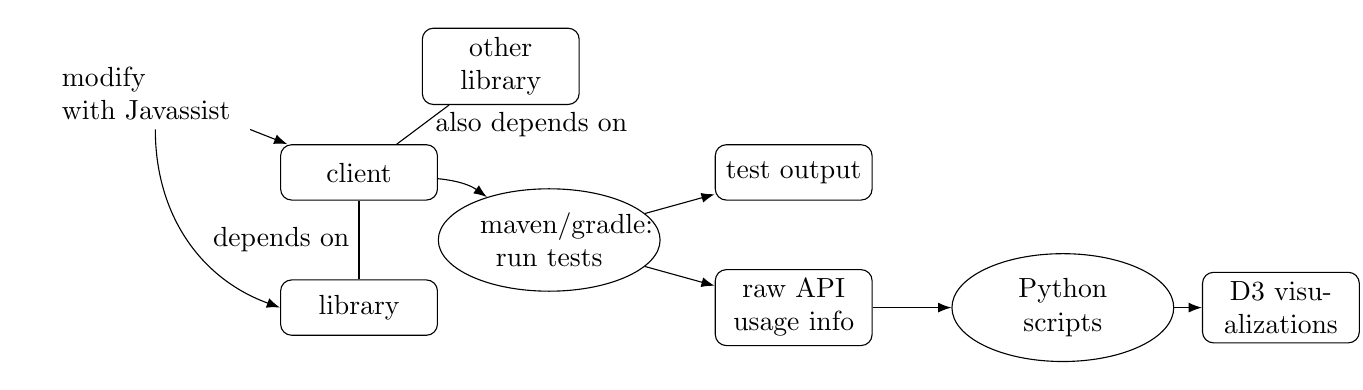
\begin{tikzpicture}
    \node[block] (client) {client};
    \node[block,below=1cm of client] (library) {library};

    \draw (library) -- node[left] (depends) {depends on} (client);

    \node[above left=.75em of client] (ja) {\begin{minipage}{7em} modify \\with Javassist \end{minipage}};
    \draw[-Latex] (ja) -> (client);
    \draw[-Latex] (ja) to [->,bend right=35] (library.west);

    \node[block, above right=2em of client,xshift=-2em] (olib) {other library};
    \draw (client) -- node[right,xshift=.1em] (also) {also depends on} (olib);

    \node[oval,right=of depends] (test) {maven/gradle: run tests};

    \draw[-Latex] (client) to [->,bend left=15] (test);

    \node[block, right=10em of client] (output) {test output};
    \node[block, right=10em of library] (raw) {raw API usage info};

    \draw[-Latex] (test) to (output);
    \draw[-Latex] (test) to (raw);

    \node[oval, right=of raw] (Py) {Python scripts};
    \draw[-Latex] (raw) to (Py);

    \node[block, right=1em of Py] (viz) {D3 visualizations};
    \draw[-Latex] (Py) to (viz);
  \end{tikzpicture}
}
  \caption{Our instrumentation workflow. Using Javassist, we analyze and instrument clients and run their test suites. We process the generated data with Python scripts to create D3 visualizations.}
  \label{fig:workflow}
 \end{center}
\end{figure*}

We collect data about client usages of libraries by running client
test suites under instrumentation. The instrumentation records API
uses which cross client/library boundaries, closely mirroring the API
usage patterns that we described in
Section~\ref{sec:api-usage-examples}. We use
Javassist~\cite{chiba00:_load_struc_reflec_java} to perform the
instrumentation and then the build system of each project (Maven or Gradle) to run its
tests. Figure~\ref{fig:workflow} summarizes our instrumentation and
data capture workflow. We next describe our instrumentation implementation in detail.

We identify interactions across the client/library boundaries by inspecting JAR files of
each software component to obtain a list of classes for every component. We associate classes 
and their members to components based on these lists. Since the JAR files contain source code,
we ensure that none of the library uses meant solely for unit testing are captured.


\section{API Usage Patterns}
\label{sec:patterns}

\section{Results}
\label{sec:results}



%======================================================================
\chapter{Applications}
%======================================================================
\section{Visualization}
\label{sec:visualization}
We now present the VizAPI tool, which shows visualization overviews depicting API usages---from clients to libraries, but also between libraries (including transitive dependencies). The goal of VizAPI is to provide a heuristic for developers considering the impacts of changes to libraries.

We have verified that each client uses only a small portion of each of its dependencies' API surfaces. Consider breaking changes again. GitHub provides the Dependabot tool~\cite{mullans20:_keep_depen}, which monitors for upstream changes and automatically proposes pull requests to update dependency versions. That tool may well pull in breaking changes. However, we hypothesize that, most of the time, most breaking changes will not affect most clients; it is useful for clients to know whether they are using the parts of the API surface that are subject to a particular breaking change. A client with broad dependencies on a library (uses a larger fraction of its API surface) is more likely to be affected by its changes than a client with narrow dependencies (smaller fraction). A narrow library dependency would also suggest that it would be easier to swap the library for a functionally similar replacement.

Our visualization allows developers and
researchers to visualize distribution information about how different
parts of clients use different parts of libraries. VizAPI incorporates information from static and dynamic analyses. 
We have made VizAPI publicly available\footnote{\url{https://github.com/SruthiVenkat/api-visualization-tool}}, although it is still in development.

\begin{figure}[h]
\begin{center}
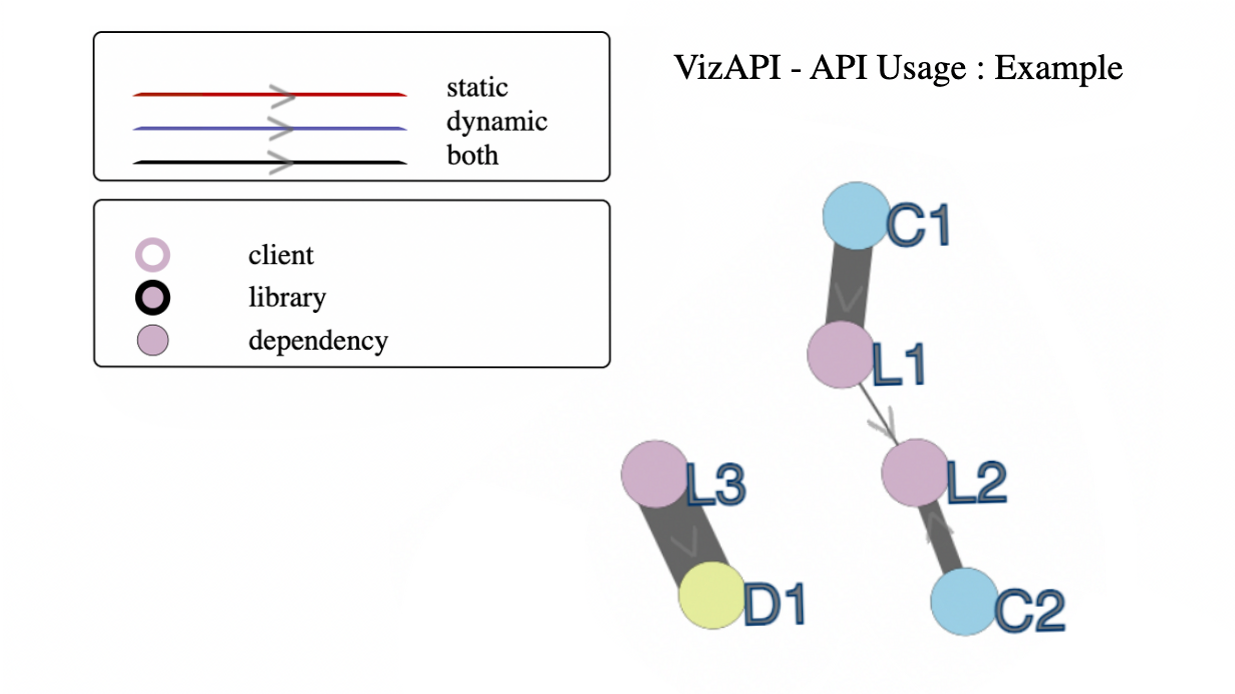
\includegraphics[height=6cm]{images/intro-example.png}
\caption{An Example VizAPI Application}
\label{fig:example}
\end{center}
\end{figure}

We first define the terms ``client'', ``library'' and ``dependency''. A ``client'' is a software component which directly uses some functionality of an external component, which is the ``library''. Any external component that the ``library'' directly uses is a ``dependency''. 

Figure~\ref{fig:example} illustrates a possible VizAPI usage scenario, from the perspective of a client developer. Consider a client $C$ (blue nodes) and a library $L$ (purple nodes), in the context of plain Java. Library $L$ has packages $L_1$, $L_2$, and $L_3$. $C$ calls into $L_1$ and $L_2$. Internally, within $L$, $L_1$ and $L_2$ call into each other, but not into $L_3$. The VizAPI result, with no edges from $C$ directly to $L_3$, allows a developer to conclude that breaking changes in $L_3$ will not affect $C$. Also, if only $L_3$ uses an external dependency $D$ (yellow node), then we know that $C$ will not need $D$ to be on its classpath.


We next describe the design of VizAPI, including how we
collect information and format it for the d3js visualization
library. We also present two VizAPI usage scenarios.

\subsection{Visualization System}
\label{subsec:vis-system}

Once we have generated data from our tool that runs the static and dynamic analyses, we use a modified version
of the d3graph\footnote{\url{https://pypi.org/project/d3graph/}} library in Python to generate a d3js\footnote{\url{https://d3js.org/}}
visualization. 
The graph in Figure~\ref{fig:usagescenario1}
is an example of a graph produced by VizAPI.

VizAPI graphs are force-directed graphs based on the frequency of
interactions between different software components.  Each node is a
set of one or more packages that belong to the same JAR.  There are
three categories of nodes: clients are represented by nodes with white
interiors; libraries by nodes with filled interiors and black borders;
and dependencies (called by libraries but not clients) by nodes with
filled interiors and normal borders.  We coalesce nodes if they
originate from the same JAR and have the same incoming and
outgoing edges.

Each edge is directed
from the source package(s) to the target package(s) and represents an interaction 
(invocations, fields, annotations, subtyping) between packages. 
The thickness of each edge reflects the frequency of interactions between the source and the target.
Double-clicking on a node emphasizes its direct interactions with other packages while fading out the rest of the graph.

We run a Python implementation of the Louvain clustering algorithm~\cite{blondel2008fast}, and make the clusters 
visible by colouring nodes based on cluster.
This means that the same colour could indicate nodes (of the same category) from the same or different JARs.
Hovering on a node shows the list of packages and 
the JAR that they belong to, 
formatted as “jar : $\langle$space separated list of packages$\rangle$”. 

\begin{figure*}[h]
\begin{center}

\subfloat[Usage Scenario 1: Library \textit{jsoup} (pink with dark borders), called by two clients, \textit{ez-vcard} (hollow with purple border) and \textit{JsoupXpath} (hollow with pink border). Exploration shows that internal jsoup packages aren't called directly by clients.
\label{fig:usagescenario1}]
{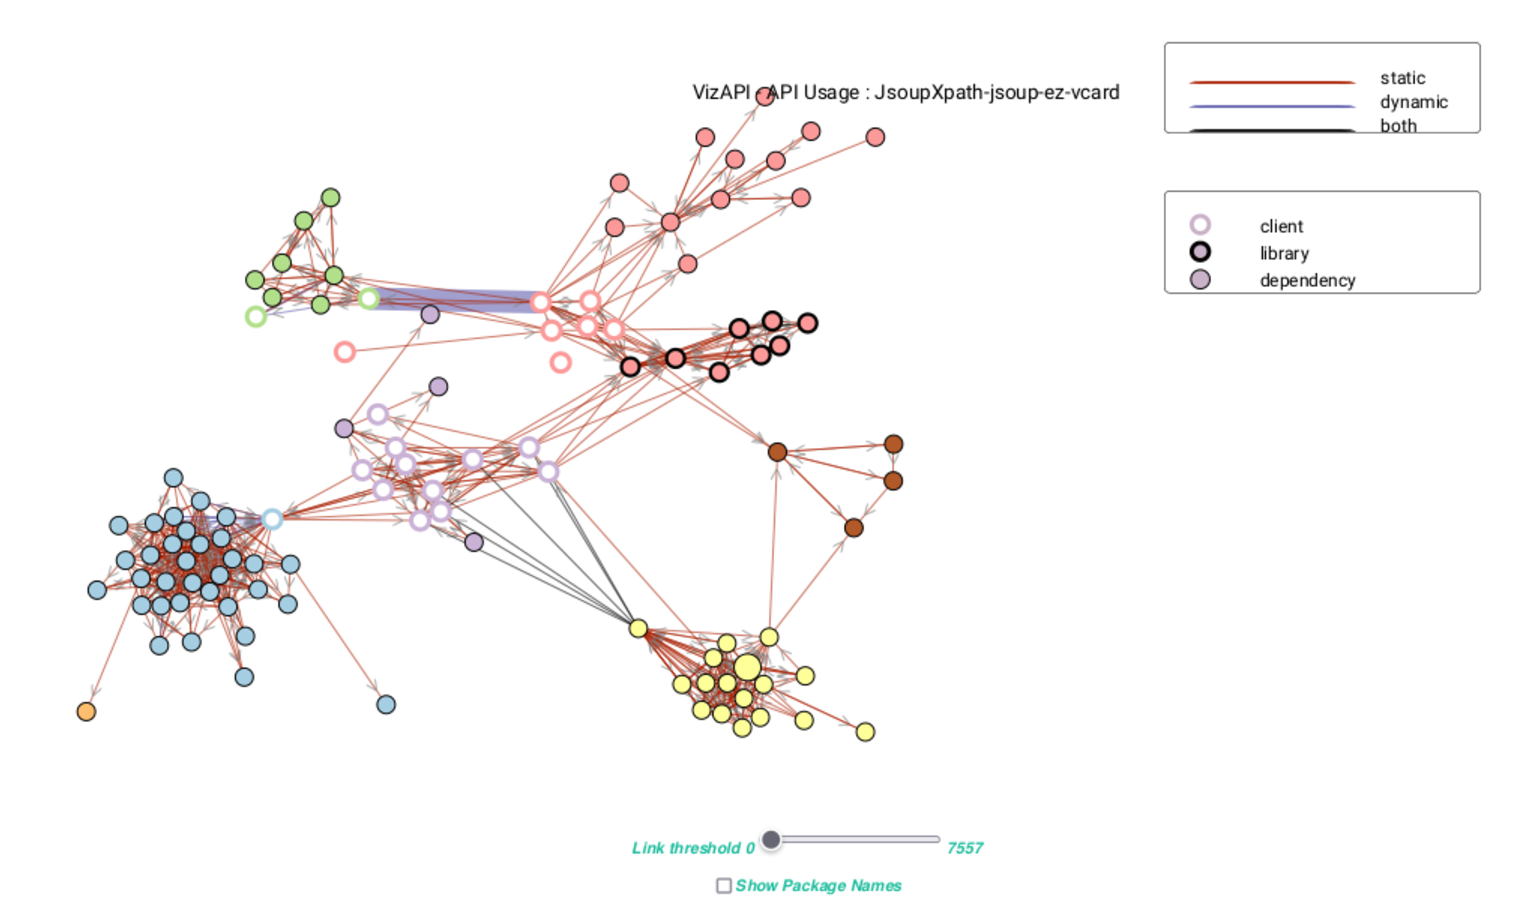
\includegraphics[width=16cm]{images/usage-scenario1.pdf}}
\hspace{7mm}

\subfloat[Usage Scenario 2: Client \textit{dataprocessor} (hollow, orange border) calls only one package in library \textit{fastjson} (green fill).
\label{fig:usagescenario2}]
{
\makebox[16cm]{
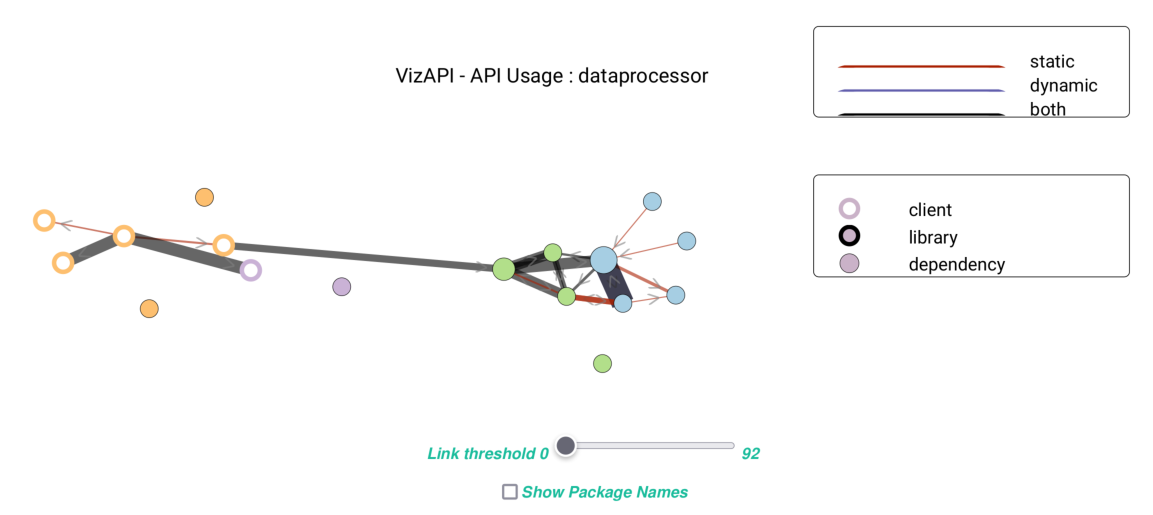
\includegraphics[width=11cm]{images/usage-scenario2.pdf}
}
}
\caption{\label{fig:usagescenarios} VizAPI Usage Scenarios.}

\end{center}
\end{figure*}


\subsection{Case Study}
\label{subsec:evaluation}

We conducted a pilot study of VizAPI.
We have generated data from our benchmarks.
We have collected both static and dynamic data for these projects, 
and we are in a position
to generate graphs for combinations of clients and libraries
in these projects. 
We present two usage scenarios below; graphs for 
our usage scenarios are publicly available.\footnote{\url{https://sruthivenkat.github.io/VizAPI-graph/}}
We intend for these usage scenarios to show how VizAPI can be useful to client developers when they want to observe library API usage and for library developers when they want to observe how their library is used by clients.

\paragraph{Usage Scenario 1: jsoup}
Imagine that we are a jsoup developer and want to understand
how some clients interact with it, in anticipation of making some breaking changes. We choose clients JsoupXpath\footnote{\url{https://github.com/zhegexiaohuozi/JsoupXpath}\label{jsoupxpath}} and ez-vcard\footnote{\url{https://github.com/mangstadt/ez-vcard}\label{ez-vcard}}.
Figure~\ref{fig:usagescenario1} shows static and dynamic interactions of the 2 clients with the jsoup\footnote{\url{https://github.com/jhy/jsoup}\label{jsoup}} library. Recall that nodes represent packages and edges represent interactions (usually invocations) between packages. 

We can start our exploration with the cluster of pink nodes. Many of these nodes belong to either JsoupXpath or jsoup. Hovering over a node tells us the package names while double-clicking shows us its direct interactions. (To search for a package, we can click on ``show package names'' and use the browser's find functionality.) Here, client JsoupXpath calls directly into \texttt{org.jsoup.nodes} and \texttt{org.jsoup.select}. Notably, and as we might expect, we can see that \texttt{org.jsoup.helper} and \texttt{org.jsoup.internal} aren't called directly by JsoupXpath. This would mean that breaking changes in \texttt{org.jsoup.helper} or \texttt{org.jsoup.internal} wouldn't directly affect JsoupXpath\footnote{As a specific example, the retraction of an internal jsoup API would not break this client. Behavioural changes that are directly passed through to the external API, e.g. through delegation, can still break clients, but we can consider those to be changes in the external API.} 

Similarly, ez-vcard, which belongs to the purple cluster in Figure~\ref{fig:usagescenario1}, directly calls into \texttt{org.jsoup}. ez-vcard also calls into jackson-core\footnote{\url{https://github.com/FasterXML/jackson-core}\label{jackson-core}} and jackson-databind\footnote{\url{https://github.com/FasterXML/jackson-databind}\label{jackson-databind}}, which are very tightly coupled amongst their own packages and with each other. As a jsoup developer, we would be indifferent; others, however, can observe that breaking changes in jackson-core and jackson-databind could propagate.

\paragraph{Usage Scenario 2: dataprocessor}

Figure~\ref{fig:usagescenario2} presents a second usage scenario. Here, say we are the developers of client dataprocessor\footnote{\url{https://github.com/dadiyang/dataprocessor}\label{dataprocessor}} (hollow with orange border). This client uses the fastjson\footnote{\url{https://github.com/alibaba/fastjson}\label{fastjson}} library (green fill). Our visualization shows calls only from dataprocessor package \texttt{com.github.dataprocessor.slice}, which is the orange-bordered client node (identity of the package available by hovering) to the package \texttt{com.alibaba.fastjson}. No other parts of dataprocessor use fastjson. This means that when we, as dataprocessor developers, need to upgrade the fastjson version, we only need to inspect the source code in our \texttt{com.github.dataprocessor.slice} package. 

Note also the disconnected nodes in Figure~\ref{fig:usagescenario2}. These are all packages of fastjson that are not used by dataprocessor: any breaking changes in these packages definitely do not directly affect dataprocessor, and are less likely to affect it overall than packages that are directly used.

We have presented a case study on possible usage scenarios for the VizAPI tool to show its usefulness to component developers and researchers.

\section{Library Fission}
Modern software uses libraries extensively, to reuse functionality. Over time, libraries tend to extend their functionality, introduce more features and modify existing ones. This could lead to huge library sizes, a lot of which goes unused by a client that imports it. This is called software bloating and there has been work around debloating. Debloating focuses on the client’s execution and analyzing the client. We propose library fission, which focuses on splitting libraries based on client usage. This is a more permanent solution to bloating and does not require running analyses on clients for every execution. (We aim to split libraries based on client behaviour in a way that sub-modules of the fissioned library have common functionality.)

We use the data generated by our static and dynamic analyses to experiment with fissioning a subset of our corpus of libraries. The following are the steps we follow to perform library fission for a given library, $L$:
\begin{enumerate}
\item Filter out all interactions with $L$, i.e., client uses of $L$, $L$'s uses of dependencies and intra-library uses of $L$.
\item Run the Louvain clustering algorithm on the filtered data where each node is set to be a package belonging to a jar.
\item Split up $L$ into Maven submodules based on the clusters.
\item Test on a subset of $L$'s clients.
\end{enumerate}

We now discuss specific examples from our libraries.

\subsection{\emph{fastjson}}
We have 26 clients for \emph{fastjson}. Based on the usages of these clients, we obtained the following initial set of 5 clusters:
\begin{enumerate}
\item Cluster 1:
\begin{itemize}
\item \texttt{com.alibaba.fastjson.annotation}
\item \texttt{com.alibaba.fastjson.asm}
\item \texttt{com.alibaba.fastjson.parser}
\item \texttt{com.alibaba.fastjson.serializer}
\item \texttt{com.alibaba.fastjson.support.hsf}
\item \texttt{com.alibaba.fastjson.support.config}
\item \texttt{com.alibaba.fastjson.support.retrofit}
\item \texttt{com.alibaba.fastjson.support.springfox}
\end{itemize}
\item Cluster 2:
\begin{itemize}
\item \texttt{com.alibaba.fastjson}
\end{itemize}
\item Cluster 3:
\begin{itemize}
\item \texttt{com.alibaba.fastjson.util}
\item \texttt{com.alibaba.fastjson.parser.deserializer}
\end{itemize}
\item Cluster 4:
\begin{itemize}
\item \texttt{com.alibaba.fastjson.support.spring}
\item \texttt{com.alibaba.fastjson.support.spring.annotation}
\end{itemize}
\item Cluster 5:
\begin{itemize}
\item \texttt{com.alibaba.fastjson.support.jaxrs}
\end{itemize}
\end{enumerate}

We observe that the clusters are loosely based on functionality, that is, the packages within a cluster have similar functionality. This is not strictly true for all packages, but it is a good approximation. We see that the \texttt{jaxrs} and \texttt{spring} functionalities are clusters of their own and it makes sense to separate these into submodules since they provide their own independent functionality. However, we observed that there exist cyclic dependencies between Cluster 1, 2 and 3. If a library developer performs library fission and they run into cyclic dependencies, we recommend that they resolve these dependencies by moving classes into appropriate submodules. Due to our lack of domain knowledge, that is knowledge about functionalities of individual classes, we combined these 3 clusters into one submodule. Our final submodules are as follows:
\begin{enumerate}
\item Submodule 1 --- utils:
\begin{itemize}
\item \texttt{com.alibaba.fastjson.annotation}
\item \texttt{com.alibaba.fastjson.asm}
\item \texttt{com.alibaba.fastjson.parser}
\item \texttt{com.alibaba.fastjson.serializer}
\item \texttt{com.alibaba.fastjson.support.hsf}
\item \texttt{com.alibaba.fastjson.support.config}
\item \texttt{com.alibaba.fastjson.support.retrofit}
\item \texttt{com.alibaba.fastjson.support.springfox}
\item \texttt{com.alibaba.fastjson}
\item \texttt{com.alibaba.fastjson.util}
\item \texttt{com.alibaba.fastjson.parser.deserializer}
\end{itemize}
\item Submodule 2 --- spring:
\begin{itemize}
\item \texttt{com.alibaba.fastjson.support.spring}
\item \texttt{com.alibaba.fastjson.support.spring.annotation}
\end{itemize}
\item Submodule 3 --- jaxrs:
\begin{itemize}
\item \texttt{com.alibaba.fastjson.support.jaxrs}
\end{itemize}
\end{enumerate}

When we split \emph{fastjson} into submodules, we observed that each submodule needed fewer dependencies in the pom compared to the current version of \emph{fastjson} that is not split. The current version of \emph{fastjson} has 61 dependencies, while \emph{utils} has 47, \emph{spring} has 27 and \emph{jaxrs} has 29. Importing one of these submodules means a lesser probability of propagated vulnerabilities, version conflicts and breaking changes.

We sent an email to the \emph{fastjson} contributors proposing a split and did not receive a response, after which we created a pull request\footnote{\url{}https://github.com/alibaba/fastjson/pull/4276}. Our PR text was as follows:
``This PR splits fastjson into 3 submodules - utils, spring, jaxrs. We're looking into Java API usage as part of research and propose this split. These submodules are based on usage patterns that we've observed clients making of fastjson. It is beneficial to clients – they can import only the submodule they need to use (utils seems to be most popular). After this change, clients will not be affected by breaking changes in unused submodules and can avoid version conflicts and vulnerabilities propagated through dependencies. We believe that this split makes it easier to release backward compatible versions of fastjson and to isolate breaking changes."

\subsection{\emph{jsoup}}
Based on usage by the 7 clients of jsoup we have in our benchmark set, we observed the following clusters:
\begin{enumerate}
\item Cluster 1:
\begin{itemize}
\item \texttt{org.jsoup.parser}
\item \texttt{org.jsoup.safety}
\item \texttt{org.jsoup.helper}
\item \texttt{org.jsoup.internal}
\end{itemize}
\item Cluster 2:
\begin{itemize}
\item \texttt{org.jsoup}
\item \texttt{org.jsoup.examples}
\end{itemize}
\item Cluster 3:
\begin{itemize}
\item \texttt{org.jsoup.select}
\item \texttt{org.jsoup.nodes}
\end{itemize}
\end{enumerate}

We observed multiple cyclic dependencies. In the case of cyclic dependencies, it is best for the library developers to split classes in packages and move them to clusters based on functionality. 

We now discuss a few interesting things we noted in the \emph{jsoup} clusters. Cluster 1 contains \texttt{org.jsoup.internal}. It is clear from the naming that this package is meant for internal use only and not for clients. We suggest that such packages be moved to a separate submodule so that clients need not import it. Similarly, Cluster 2 contains \texttt{org.jsoup.examples} which also almost certainly will not be needed by clients and can also be moved to a separate submodule. 

Due to the multiple cyclic dependencies that we observed, we did not raise a pull request for \emph{jsoup}.

\section{Upgrades, Breaking Changes and Backward Compatibility}
Our data for 101 Java software components contains different kind of interactions across component boundaries. This data can be analyzed and prove useful in the following ways:
\begin{itemize}
\item Library developers can observe different usage patterns of their APIs. The clusters observed in library packages can help with new version releases. Breaking changes might be restricted to clusters and library developers can choose whether to make clusters from new versions backward compatible with other clusters from older versions or not. 
\item Clients can also check if breaking changes in new library versions will affect their code during upgrades. 
\item Unused dependencies can be identified and removed to prevent them from possibly introducing version conflicts and vulnerabilties.
\end{itemize}

%%======================================================================
\chapter{Methodology}
%======================================================================


%%======================================================================
\chapter{Results and Discussion}
%======================================================================


%======================================================================
\chapter{Conclusion}
\label{sec:conclusion}
%======================================================================
The goal of this work was to enable 1) library developers to make better
decisions when designing new APIs, pruning or modifying unused APIs and to refactor their
libraries; and 2) client developers to make better decisions about library
upgrades and breaking changes.

Further user evaluations of our VizAPI tool can establish and improve the
effectiveness of VizAPI. This can be performed following
existing techniques~\cite{merino18:_system_liter_review_softw_visual_evaluat}; in
particular, experiments, where users perform software
understanding and maintenance tasks.


\section{Threats to Validity}
Our threats to validity include the usual threat to external validity
of insufficient sample size or variety---many of our seed libraries
are JSON parser/generators, although our transitive closures result in
a wider range of domains.

There is also the construct validity issue that tests may
not adequately represent actual client behaviours. However, our use of both static
and dynamic information addresses this issue. Specifically, because we use
class hierarchy analysis for our static analysis, our visualization will present
all possible static calls---possibly too many. 
That is, the main hazard with static analysis is that our visualization may include more
static edges than are actually possible. Some of those edges could be ruled out by a more
precise call graph. Reflection aside, no static edges
are missing (our approach is ``soundy''~\cite{livshits15:_in_defen_sound} with respect to static information). On the other hand, dynamic edges have actually been observed
on some execution; better tests could yield more dynamic edges. But even if
a dynamic edge is missing, there will be a static edge if the behaviour is possible.

We may have missed other categories of bypass patterns---though we believe
that we have chosen at least a representative sample of mechanisms to ensure
modularity. 

Finally, our results apply best to Java-like languages, and
may vary dramatically for other languages.

\section{Actionable Outcomes}
Based on our exploration of API uses and mis-uses, we make some recommendations
for both API and language/analysis designers.

\begin{enumerate}
\item API scope: given that both we and Thummalapenta and Xie~\cite{thummalapenta08:_spotw} find
that APIs are sparsely used, API designers can seek to prune unused APIs;
\item Refactoring: our results show that library fission is useful, i.e., some existing APIs can be split into loosely-connected parts, reducing effective API surface and potentially developer cognitive burden;
\item Deprecation: one could investigate the scope for aggressive deprecation of unused APIs in released libraries, giving more liberty to API designers to modify their code;
\item Modularity: API and language designers can be confident that stated encapsulation boundaries are respected.
\end{enumerate}
%Encapsulation is a fundamental building block for software systems. API boundaries are an important way to enforce encapsulation, and our results show how developers interact with API boundaries in practice.

%% \item Automatically enforce encapsulation boundaries i.e. flag code that does things it shouldn't.
%% \begin{enumerate}
%% \item Upstream can provide wider published APIs if needed
%% \item Downstream can refactor to use narrower APIs if required
%% \item Can provide shims for downstream to use until upstream widens.
%% \end{enumerate}
%% \item Restrict the declared API to an actually-used subset and support deprecation of unused API bits.
%% \end{enumerate}

We studied API usage in detail in this work and explored its usefulness by presenting two developer-focussed applications of it. We found that clients do not access internal parts of libraries for the most part. We also found that clients use only a small part of existing APIs and also that different clients use different parts of libraries with only a small overlap. This result makes a case for library fission, which we observed has the benefits of reduced dependencies in an application. We also presented the VizAPI visualization tool, which can be used by developers to observe API usage in their components.

%----------------------------------------------------------------------
% END MATERIAL
%----------------------------------------------------------------------

% B I B L I O G R A P H Y
% -----------------------

% The following statement selects the style to use for references.  It controls the sort order of the entries in the bibliography and also the formatting for the in-text labels.
\bibliographystyle{plain}
% This specifies the location of the file containing the bibliographic information.  
% It assumes you're using BibTeX (if not, why not?).
\cleardoublepage % This is needed if the book class is used, to place the anchor in the correct page,
                 % because the bibliography will start on its own page.
                 % Use \clearpage instead if the document class uses the "oneside" argument
\phantomsection  % With hyperref package, enables hyperlinking from the table of contents to bibliography             
% The following statement causes the title "References" to be used for the bibliography section:
\renewcommand*{\bibname}{References}

% Add the References to the Table of Contents
\addcontentsline{toc}{chapter}{\textbf{References}}

\bibliography{uw-ethesis}
% Tip 5: You can create multiple .bib files to organize your references. 
% Just list them all in the \bibliogaphy command, separated by commas (no spaces).

% The following statement causes the specified references to be added to the bibliography% even if they were not 
% cited in the text. The asterisk is a wildcard that causes all entries in the bibliographic database to be included (optional).
\nocite{*}

% The \appendix statement indicates the beginning of the appendices.
\appendix
% Add a title page before the appendices and a line in the Table of Contents
\chapter*{APPENDICES}
\addcontentsline{toc}{chapter}{APPENDICES}
%======================================================================
\chapter[PDF Plots From Matlab]{Matlab Code for Making a PDF Plot}
\label{AppendixA}
% Tip 4: Example of how to get a shorter chapter title for the Table of Contents 
%======================================================================
\section{Using the GUI}
Properties of Matab plots can be adjusted from the plot window via a graphical interface. Under the Desktop menu in the Figure window, select the Property Editor. You may also want to check the Plot Browser and Figure Palette for more tools. To adjust properties of the axes, look under the Edit menu and select Axes Properties.

To set the figure size and to save as PDF or other file formats, click the Export Setup button in the figure Property Editor.

\section{From the Command Line} 
All figure properties can also be manipulated from the command line. Here's an example: 
\begin{verbatim}
x=[0:0.1:pi];
hold on % Plot multiple traces on one figure
plot(x,sin(x))
plot(x,cos(x),'--r')
plot(x,tan(x),'.-g')
title('Some Trig Functions Over 0 to \pi') % Note LaTeX markup!
legend('{\it sin}(x)','{\it cos}(x)','{\it tan}(x)')
hold off
set(gca,'Ylim',[-3 3]) % Adjust Y limits of "current axes"
set(gcf,'Units','inches') % Set figure size units of "current figure"
set(gcf,'Position',[0,0,6,4]) % Set figure width (6 in.) and height (4 in.)
cd n:\thesis\plots % Select where to save
print -dpdf plot.pdf % Save as PDF
\end{verbatim}

\end{document}
